\section{Lernziele (Leitfragen) SW 06}
\begin{itemize}
    \item How do I find out my IPv4 configuration?
    \item How do I find the IP address associated to a URL?
    \item How do I determine if a host is “up” given its IP or URL?
    \item How do I find out which intermediate network devices are there between my host and another host, given its IPv4 address (or URL)?
    \item Wieso brauchen wir IPv6? Was sind die Nachteile von IPv4?
    \item Wie lange sind IPv6 Adressen?
    \item Was sind die Regeln, um eine IPv6 Adresse zu komprimieren?
    \item Wie sind IPv6 Adressen unterteilt?
    \item Was für IPv6 unicast Adress Arten gibt es?
    \item Über welche IPv6 unicast Adressen sollte ein richtig konfigurierte Host mindestens verfügen?
    \item Wie sind IPv6 Global Unicast Addresses (GUAs) unterteilt?
    \item Welche Mechanismen werden verwendet, um IPv4 und IPv6 Netzwerken miteinander zu verbinden?
\end{itemize}

\section{Antworten}
\subsection*{How do I find out my IPv4 configuration?}
\begin{multicols}{2}
    Windows: \texttt{ipconfig [/all]}
    \begin{figure}[H]
        \begin{center}
        \label{pic:ipconfig}
        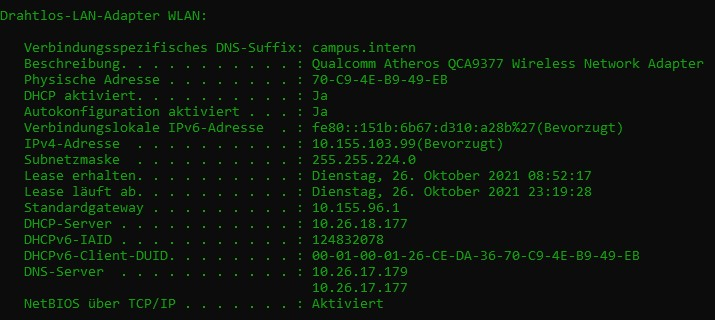
\includegraphics[width=.5\textwidth]{images/ipconfig.jpg}
        \caption{Adapterkonfiguration in Windows mit \texttt{ipconfig /all}}
        \end{center}
    \end{figure}
    \columnbreak
    Unix: \texttt{ifconfig}
    \begin{figure}[H]
        \begin{center}
        \label{pic:ifconfig}
        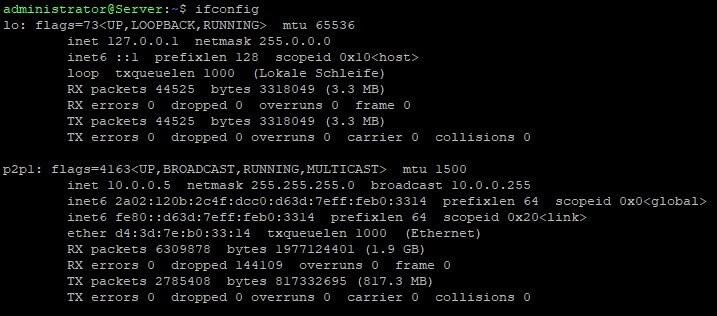
\includegraphics[width=.5\textwidth]{images/ifconfig.jpg}
        \caption{Adapterkonfiguration in Ubuntu mit \texttt{ifconfig}}
        \end{center}
    \end{figure}
\end{multicols}
\subsection*{How do I find the IP address associated to a URL?}
\begin{multicols}{2}
    \texttt{nslookup <URL>}
    \begin{figure}[H]
        \begin{center}
        \label{pic:nslookup_win{Sprungmarke}}
        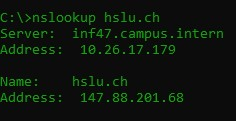
\includegraphics[width=.5\textwidth]{images/nslookup_win.jpg}
        \caption{\texttt{nslookup} in Windows}
        \end{center}
    \end{figure}
    \columnbreak
    \vfill\null
    \begin{figure}[H]
        \begin{center}
        \label{pic:nslookup_unix}
        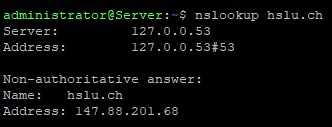
\includegraphics[width=.5\textwidth]{images/nslookup_unix.jpg}
        \caption{\texttt{nslookup} in Ubuntu}
        \end{center}
    \end{figure}
\end{multicols}
\pagebreak
\subsection*{How do I determine if a host is “up” given its IP or URL?}
\begin{multicols}{2}
    Windows:
    \begin{itemize}
        \item \texttt{ping [-4] <URL>}
        \item \texttt{ping <IPv4-Adresse>}
    \end{itemize}
    \begin{figure}[H]
        \begin{center}
        \label{pic:ping_win}
        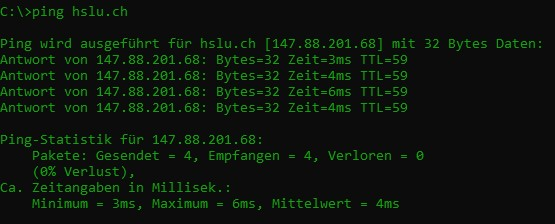
\includegraphics[width=.5\textwidth]{images/ping_win.jpg}
        \caption{\texttt{ping} in Windows}
        \end{center}
    \end{figure}
    \columnbreak
    Unix: \texttt{ping <IPv4-Adresse | URL>} (Ctrl+C zum abbrechen)
    \vfill\null
    \begin{figure}[H]
        \begin{center}
        \label{pic:ping_unix}
        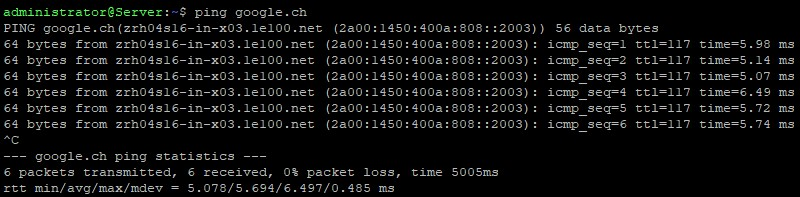
\includegraphics[width=.5\textwidth]{images/ping_unix.jpg}
        \caption{\texttt{ping} in Ubuntu}
        \end{center}
    \end{figure}
\end{multicols}
\subsection*{How do I find out which intermediate network devices are there between my host and another host, given its IPv4 address (or URL)?}
\begin{multicols}{2}
    Windows:
    \begin{itemize}
        \item \texttt{tracert [-4] <URL>}
        \item \texttt{tracert <IPv4 Address>}
    \end{itemize}
    \begin{figure}[H]
        \begin{center}
        \label{pic:tracert}
        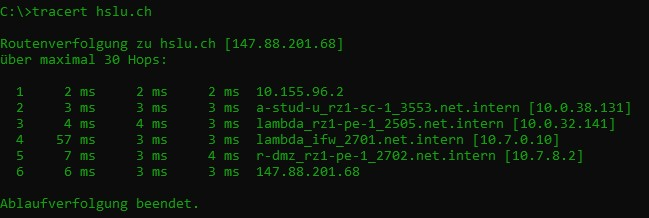
\includegraphics[width=.5\textwidth]{images/tracert.jpg}
        \caption{\texttt{tracert} in Windows}
        \end{center}
    \end{figure}
    %\vfill\null
    \columnbreak
    Unix: \texttt{traceroute <IPv4 Adress | URL>}
    \begin{figure}[H]
        \begin{center}
        \label{pic:traceroute}
        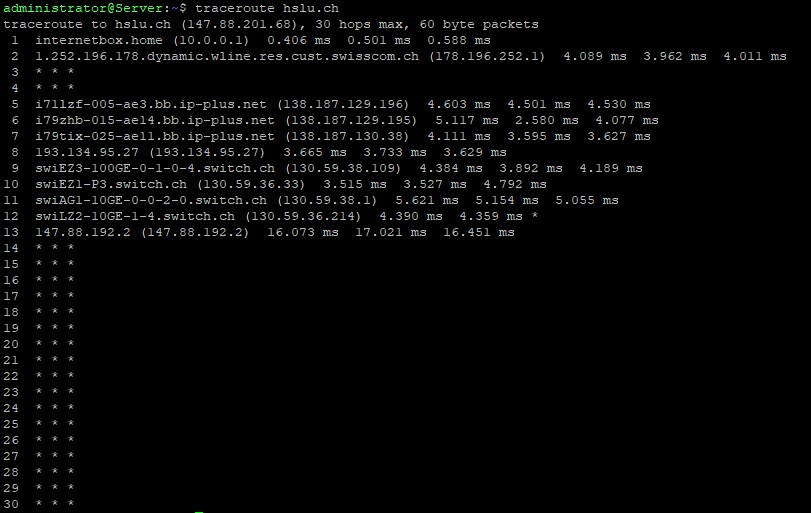
\includegraphics[width=.5\textwidth]{images/traceroute.jpg}
        \caption{\texttt{traceroute} in Ubuntu}
        \end{center}
    \end{figure}
\end{multicols}

\subsection*{Wieso brauchen wir IPv6? Was sind die Nachteile von IPv4?}
//TODO
\subsection*{Wie lange sind IPv6 Adressen?}
128 bit
\subsection*{Was sind die Regeln, um eine IPv6 Adresse zu komprimieren?}
//TODO
\subsection*{Wie sind IPv6 Adressen unterteilt?}
//TODO
\subsection*{Was für IPv6 unicast Adress Arten gibt es?}
//TODO
\subsection*{Über welche IPv6 unicast Adressen sollte ein richtig konfigurierte Host mindestens verfügen?}
\begin{itemize}
    \item 64 bit prefix
    \begin{itemize}
        \item \textbf{Global Routing Prefix}: Portion of the address that is assigned by the provider, such as an ISP, to a customer or site. The global routing prefix will vary depending on ISP policies.
        \item \textbf{Subnet ID}: Portion between the Global Routing Prefix and the Interface ID. The Subnet ID is used by an organization to identify subnets within its site.
    \end{itemize}
    \item Interface ID: Equivalent to the host portion of an IPv4 address.
\end{itemize}
\subsection*{Wie sind IPv6 Global Unicast Addresses (GUAs) unterteilt?}
//TODO
\subsection*{Welche Mechanismen werden verwendet, um IPv4 und IPv6 Netzwerken miteinander zu verbinden?}
\begin{enumerate}
    \item Dual stack - The devices run both IPv4 and IPv6 protocol stacks simultaneously.
    \item Tunneling - A method of transporting an IPv6 packet over an IPv4 network. The IPv6 packet is encapsulated inside an IPv4 packet.
    \item Translation - Network Address Translation 64 (NAT64) allows IPv6-enabled devices to communicate with IPv4-enabled devices using a translation technique similar to NAT for IPv4.
\end{enumerate}